\documentclass[tikz]{standalone}
\usepackage{pgfplots}
\pgfplotsset{compat=1.15}
\usepackage{mathrsfs}
\usetikzlibrary{arrows,calc}
\usepackage{tkz-euclide}

\pagestyle{empty}

\definecolor{AngleClr}{rgb}{0,0.39215686274509803,0}
\definecolor{ShapeClr}{rgb}{0.6,0.2,0}
\definecolor{SecondAngleClr}{RGB}{14, 70, 161}

\begin{document}

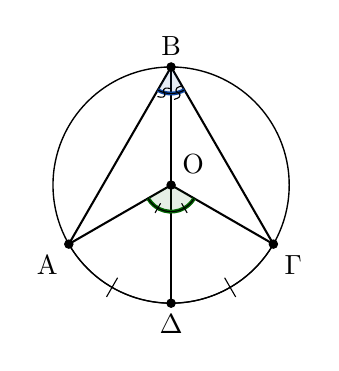
\begin{tikzpicture}[scale=.75]
\tkzSetUpLine[line width=1pt,color=black]
\tkzSetUpPoint[fill=black]

\tkzDefPoints{0/0/O,2/0/X}

\tkzDefPoint(-30:2){C}
\tkzDefPoint(210:2){A}
\tkzDefPoint(90:2){B}
\tkzDefPoint(270:2){D}

\tkzDrawCircle[color=black,fill=white,line width=0.5pt](O,X)

\tkzDrawSegments[line width=0.75pt,color=black](A,B C,B O,A O,C B,D)

\tkzFillAngles[fill=SecondAngleClr,size=.45,fill opacity=0.1](A,B,C)
\tkzMarkAngles[line width=1.4pt,size=.45,color=SecondAngleClr](A,B,C)

\tkzFillAngles[fill=AngleClr,size=.45,fill opacity=0.1](A,O,C)
\tkzMarkAngles[line width=1.4pt,size=.45,color=AngleClr](A,O,C)
\tkzMarkAngles[size=.45,mark=|,mksize=2](A,O,D D,O,C)
\tkzMarkAngles[size=.45,mark=s,mksize=2](A,B,D D,B,C)

\tkzDrawPoints[size=3](A,B,C,D,O)

\tkzLabelPoint[below left](A){$\rm A$}
\tkzLabelPoint[above](B){$\rm B$}
\tkzLabelPoint[below right](C){$\rm\Gamma$}
\tkzLabelPoint[below](D){$\rm\Delta$}
\tkzLabelPoint[above right](O){$\rm O$}

\tkzMarkAngles[size=2,mark=|](A,O,D D,O,C)

\end{tikzpicture}

\end{document}
